\section{Method}
%Paragraph one: Overview of the method. What are the high level steps taken to build the system? What are the key techniques used within the system?
We build a split error classifier using a convolutional neural network (CNN) to scan the boundaries of an existing automatic segmentation (for which there are many methods \cite{jain2010,kaynig13,Liu2014,NunezIglesias2013Machine,GALA2014,amelio_segmentation}). For each boundary, our classifier provides a probability that points sampled along the boundary caused a split error. These samples are then combined into a final edge score. Correcting a split error is as simple as merging the two bordering labels, either automatically based on a score threshold, or through highlighting a likely error boundary to the user.

Identification and correction of merge errors is slower and more challenging, because we must look inside segmentation regions for missing or incomplete boundaries, and then propose the correct boundary. However, we can reuse the same trained CNN for this task. For each segmentation label, we generate 30 potential boundaries through the region by placing seed points to a watershed cut along the opposite edges of the label boundary. Then, we check to see whether any potential edge is classified a split error as before. If the CNN detects a boundary with a very low split error score, then the boundary should have been in the segmentation and the region is a candidate for a merge error.

\begin{figure}[t]
\centering
\includegraphics[scale=.15]{gfx/patches.pdf}
\caption{Show visually each of the inputs to the system on a couple of patches.}
\end{figure}


\subsection{Network Design}
%Paragraph: What is the rationale behind our network design? Why do we think this will work over other approaches?
One typical way to train a CNN for boundary detection is to take in a wide context of the boundary in the decision making process. This is accomplished by passing in as inputs to the CNN the outputs of an automatic segmentation method windowed around a particular decision point or pixel: the input grayscale image patch, the corresponding boundary probability map patch, and two corresponding binary mask patches for the regions either side of the boundary. Following Bogovic et al.~\cite{BogovicHJ13}, these two masks can be combined into a single mask with comparable performance. The network then leverages these multiple input patches to identify and correct errors made by the previous membrane detection network and automatic segmentation pipeline.

One classic way to combine these inputs is to treat them as a 3-channel input, so that alignment between the input image and the segmentation masks are not lost throughout the convolutions. However, training a boundary-classifying network can be difficult due to rigid ground-truth segmentations, which often differ substantially from automatic segmentation regions in ambiguous intercellular space. To cope with this variation, instead our network is based on multiple separate input channels (Fig.~\ref{fig:layers}). Each of the input patches is connected individually to a 2-layer network, with each layer consisting of convolutional and pooling layers. The output of these networks is then combined by a fully connected multi-layer perceptron (MLP) with one hidden layer and a two class logistic regression output layer. The intuition for this multiple input channel approach is that we want to allow variation in the input and masks independently, to accommodate potential error, and then for the hidden layers to discover appropriate combinations of the relevant features learned separately for the different input channels.

\VKF{DELETE RIGHT? Another change is in the pooling layer itself. Bogovic et al.~\cite{BogovicHJ13} designed an unsupervised learning approach for agglomerative clustering of oversegmentations, using dynamic pooling of features extracted around objects and boundaries to increase performance. Inspired by their call for a supervised learning equivalent, we integrate a pooling layer into our CNN which is similar in spirit to their unsupervised approach. Instead of conventional max- or avg-pooling where a sliding window is equally applied to the whole output of the convolutional layer, our dynamic pooling only averages outputs within a region of interest. We implemented both pooling methods and compared them ???} 

\begin{figure}[t]
 \centering
    \subfloat[CNN Layers\label{fig:layers}]{%
      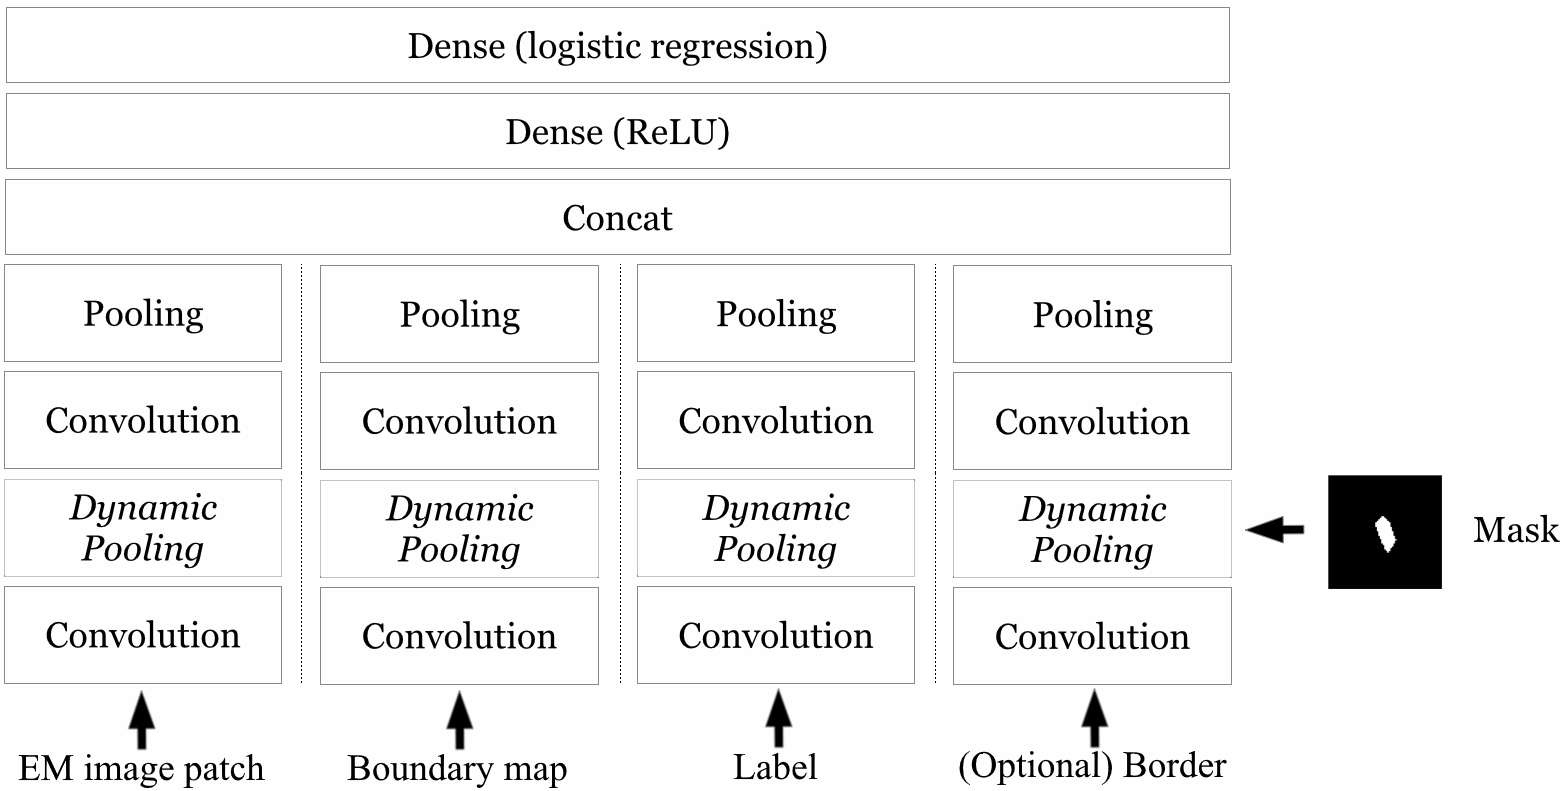
\includegraphics[width=0.55\textwidth]{gfx/layers_jt.png}
    }
    \hfill
    \subfloat[Network configurations\label{fig:networks}]{%
      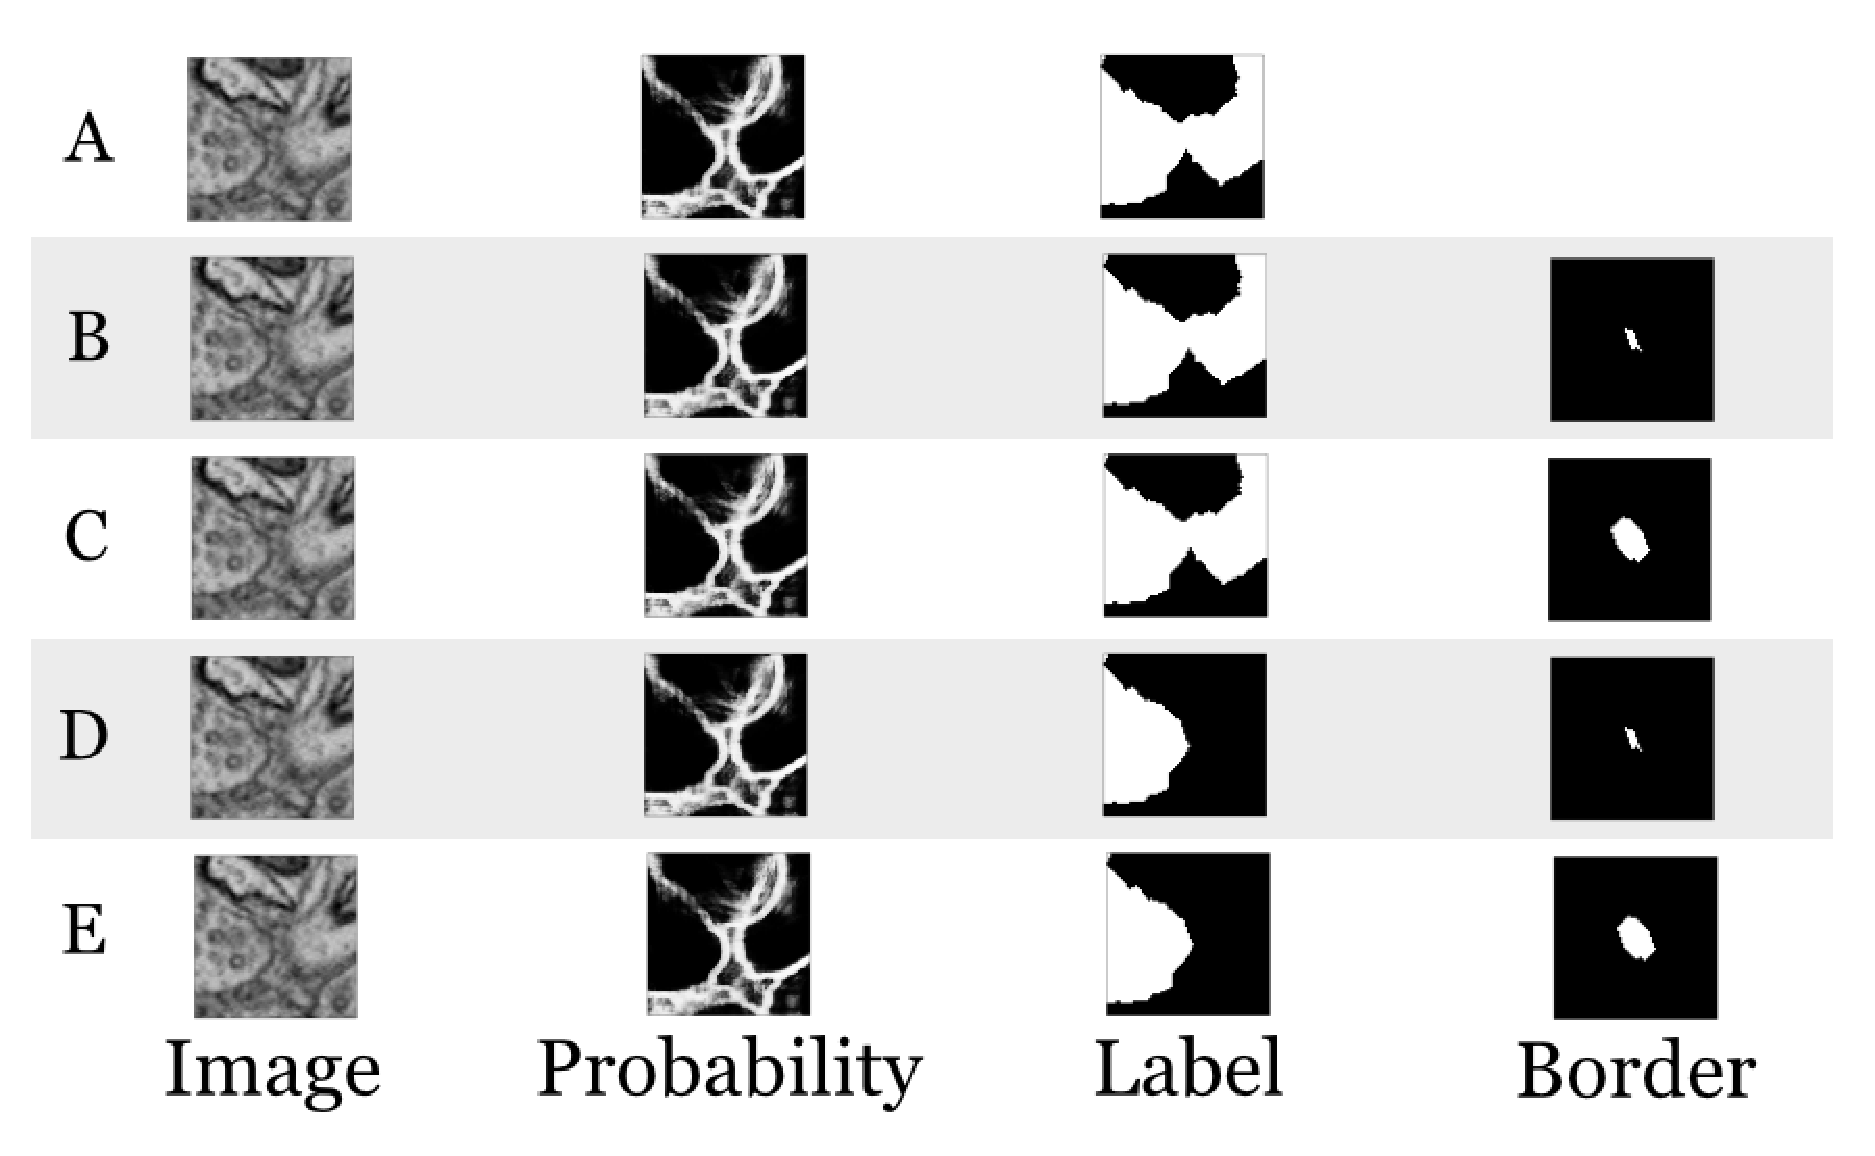
\includegraphics[width=0.4\textwidth]{gfx/networks.pdf}
    }
	\caption{a) Our proposed network architecture with up to four input channels. Each input channel involves two convolutional and two pooling layers, where the first is a dynamic pooling layer inspired by Bogovic et al.~\cite{BogovicHJ13}. b) We trained five different network configurations with three and four inputs: A) image, boundary map probability, and merged binary mask, B) extended with a small border mask, C) extended with a large border mask and D)+E) using a single label binary mask instead of the merged one with the small and large border mask.}
\end{figure}
%  
%    \begin{subfig}[b]{0.5\textwidth}
%        \includegraphics[scale=.15]
%        \caption{CNN Layers}
%        \label{fig:layers}
%    \end{subfigure}
%    \begin{subfigure}[b]{0.5\textwidth}
%        \includegraphics[scale=.15]
%        \caption{Different Network Configurations}
%        \label{fig:networks}
%    \end{subfigure}    
%\missingfigure{Network architecture figure}


\subsection{Training}
To train the network, we use a mouse cortex data set (1024x1024x75 pixels). The tissue is dense mammalian neuropil from layers 4 and 5 of the S1 primary somatosensory cortex of a healthy mouse. The resolution of our data set is $6nm$ per pixel, and the section thickness is $30nm$. \VKF{For the initial automatic segmentation, we train an existing pipeline on a similar data set}. Manually-labeled expert segmentation was available as a ground truth for the entire data set \JT{citation? URL?}. We use the first 65 sections of the data for training, the next 5 for validation, and the last 5 for testing.
%#   Training data:
%#   Patch size: (75,75)
%#   79828 correct splits
%#   79828 split errors
%#   rotated 90,180,270 degrees after each epoch
%
%#   validation data: 7464 correct splits + 7464 split errors
%#   test data: 5748 correct splits + 5748 split errors

\JT{Up to here.}
To generate training data, identify correct regions and split errors in the automatic segmentation by comparing the overlap with the ground truth regions. From these regions we sample 79828 correct regions and 79828 split error patches.

We train our network using the following parameters: learning rate $lr=.00001$, momentum $m=.9$, filter size $fs=13x13$ and number of filters $fn=16$. We assume that the training has converged if the validation loss does not decrease for 30 epochs. The network is specified using the deep learning libraries Lasagne and Theano, and trained on a Tesla K40m graphics card. 

\subsection{Automatic Error Correction}
Cell boundaries are rated by our first classifier as correct ($p=0$) or split errors ($p=1$) using the direct CNN probability score. A greedy algorithm then merges neighboring regions sequentially, starting with the highest probability scores. Following each merge, neighboring boundaries need to be re-evaluated. \VKF{Our experiments have shown that the best average probability threshold to stop this process is in the range ($p_t=.7-1.0$) not sure what to do with this, I think this is from the test data? Do we need this still? At the moment it sounds weird}.

Our second classifier identifies merge errors by using the inverse score of the trained network for split error detection. For this, we generate many possible splits in a given label using randomly seeded watershed on the inverted grayscale EM image as shown in figure \ref{fig:merge_error}. \VKF{Do we need this? If it stays we should not just hope. I think it can go if we publish the code. Further, we dilate the label by a fixed amount ($d=20$) prior to running watershed, hoping that one of the generated split edges clings to the boundary of the cell and then follows the correct splitting edge. To remove pixels which then match the boundary of the cell, we perform erosion by a fixed amount ($e=5$).} 

\begin{figure}[t]
\centering
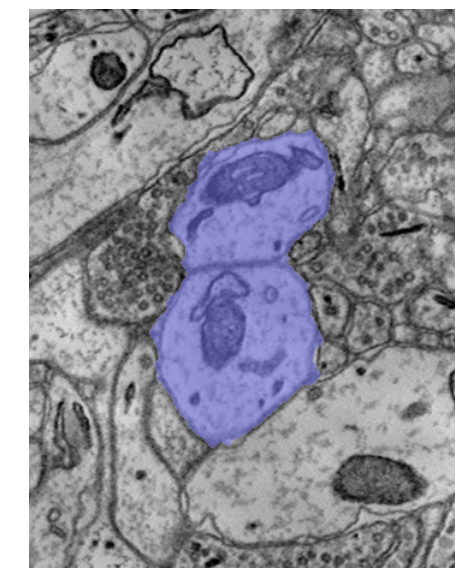
\includegraphics[scale=.22]{gfx/mergeerror.pdf}
\caption{Merge error detection and correction using our classifier: Possible boundaries are generated and rated as split errors using the proposed CNN. The lowest rated boundary which has the lowest split error score, is the most likely the correct boundary.}
\label{fig:merge_error}
\end{figure}
%
%\begin{table}
%\begin{tabular}{ll}
%\toprule
%Parameter & Value \\
%\midrule
%one & \\
%two & \\
%three & \\
%\bottomrule
%\end{tabular}
%\caption{This is a table of parameters. This is not very interesting, but it's easier to read than in the body text and putting everything together helps the reader quickly assess.}
%\end{table}